% Generated by Sphinx.
\def\sphinxdocclass{report}
\documentclass[letterpaper,10pt,openany,oneside]{sphinxmanual}
\usepackage[utf8]{inputenc}
\DeclareUnicodeCharacter{00A0}{\nobreakspace}
\usepackage[T1]{fontenc}
\usepackage[english]{babel}
\usepackage{times}
\usepackage[Bjarne]{fncychap}
\usepackage{longtable}
\usepackage{sphinx}
\usepackage{multirow}


\title{Hadoop Network Analysis}
\date{August 08, 2014}
\release{}
\author{CSinParallel Project}
\newcommand{\sphinxlogo}{}
\renewcommand{\releasename}{}
\makeindex

\makeatletter
\def\PYG@reset{\let\PYG@it=\relax \let\PYG@bf=\relax%
    \let\PYG@ul=\relax \let\PYG@tc=\relax%
    \let\PYG@bc=\relax \let\PYG@ff=\relax}
\def\PYG@tok#1{\csname PYG@tok@#1\endcsname}
\def\PYG@toks#1+{\ifx\relax#1\empty\else%
    \PYG@tok{#1}\expandafter\PYG@toks\fi}
\def\PYG@do#1{\PYG@bc{\PYG@tc{\PYG@ul{%
    \PYG@it{\PYG@bf{\PYG@ff{#1}}}}}}}
\def\PYG#1#2{\PYG@reset\PYG@toks#1+\relax+\PYG@do{#2}}

\expandafter\def\csname PYG@tok@gd\endcsname{\def\PYG@tc##1{\textcolor[rgb]{0.63,0.00,0.00}{##1}}}
\expandafter\def\csname PYG@tok@gu\endcsname{\let\PYG@bf=\textbf\def\PYG@tc##1{\textcolor[rgb]{0.50,0.00,0.50}{##1}}}
\expandafter\def\csname PYG@tok@gt\endcsname{\def\PYG@tc##1{\textcolor[rgb]{0.00,0.25,0.82}{##1}}}
\expandafter\def\csname PYG@tok@gs\endcsname{\let\PYG@bf=\textbf}
\expandafter\def\csname PYG@tok@gr\endcsname{\def\PYG@tc##1{\textcolor[rgb]{1.00,0.00,0.00}{##1}}}
\expandafter\def\csname PYG@tok@cm\endcsname{\let\PYG@it=\textit\def\PYG@tc##1{\textcolor[rgb]{0.25,0.50,0.56}{##1}}}
\expandafter\def\csname PYG@tok@vg\endcsname{\def\PYG@tc##1{\textcolor[rgb]{0.73,0.38,0.84}{##1}}}
\expandafter\def\csname PYG@tok@m\endcsname{\def\PYG@tc##1{\textcolor[rgb]{0.13,0.50,0.31}{##1}}}
\expandafter\def\csname PYG@tok@mh\endcsname{\def\PYG@tc##1{\textcolor[rgb]{0.13,0.50,0.31}{##1}}}
\expandafter\def\csname PYG@tok@cs\endcsname{\def\PYG@tc##1{\textcolor[rgb]{0.25,0.50,0.56}{##1}}\def\PYG@bc##1{\setlength{\fboxsep}{0pt}\colorbox[rgb]{1.00,0.94,0.94}{\strut ##1}}}
\expandafter\def\csname PYG@tok@ge\endcsname{\let\PYG@it=\textit}
\expandafter\def\csname PYG@tok@vc\endcsname{\def\PYG@tc##1{\textcolor[rgb]{0.73,0.38,0.84}{##1}}}
\expandafter\def\csname PYG@tok@il\endcsname{\def\PYG@tc##1{\textcolor[rgb]{0.13,0.50,0.31}{##1}}}
\expandafter\def\csname PYG@tok@go\endcsname{\def\PYG@tc##1{\textcolor[rgb]{0.19,0.19,0.19}{##1}}}
\expandafter\def\csname PYG@tok@cp\endcsname{\def\PYG@tc##1{\textcolor[rgb]{0.00,0.44,0.13}{##1}}}
\expandafter\def\csname PYG@tok@gi\endcsname{\def\PYG@tc##1{\textcolor[rgb]{0.00,0.63,0.00}{##1}}}
\expandafter\def\csname PYG@tok@gh\endcsname{\let\PYG@bf=\textbf\def\PYG@tc##1{\textcolor[rgb]{0.00,0.00,0.50}{##1}}}
\expandafter\def\csname PYG@tok@ni\endcsname{\let\PYG@bf=\textbf\def\PYG@tc##1{\textcolor[rgb]{0.84,0.33,0.22}{##1}}}
\expandafter\def\csname PYG@tok@nl\endcsname{\let\PYG@bf=\textbf\def\PYG@tc##1{\textcolor[rgb]{0.00,0.13,0.44}{##1}}}
\expandafter\def\csname PYG@tok@nn\endcsname{\let\PYG@bf=\textbf\def\PYG@tc##1{\textcolor[rgb]{0.05,0.52,0.71}{##1}}}
\expandafter\def\csname PYG@tok@no\endcsname{\def\PYG@tc##1{\textcolor[rgb]{0.38,0.68,0.84}{##1}}}
\expandafter\def\csname PYG@tok@na\endcsname{\def\PYG@tc##1{\textcolor[rgb]{0.25,0.44,0.63}{##1}}}
\expandafter\def\csname PYG@tok@nb\endcsname{\def\PYG@tc##1{\textcolor[rgb]{0.00,0.44,0.13}{##1}}}
\expandafter\def\csname PYG@tok@nc\endcsname{\let\PYG@bf=\textbf\def\PYG@tc##1{\textcolor[rgb]{0.05,0.52,0.71}{##1}}}
\expandafter\def\csname PYG@tok@nd\endcsname{\let\PYG@bf=\textbf\def\PYG@tc##1{\textcolor[rgb]{0.33,0.33,0.33}{##1}}}
\expandafter\def\csname PYG@tok@ne\endcsname{\def\PYG@tc##1{\textcolor[rgb]{0.00,0.44,0.13}{##1}}}
\expandafter\def\csname PYG@tok@nf\endcsname{\def\PYG@tc##1{\textcolor[rgb]{0.02,0.16,0.49}{##1}}}
\expandafter\def\csname PYG@tok@si\endcsname{\let\PYG@it=\textit\def\PYG@tc##1{\textcolor[rgb]{0.44,0.63,0.82}{##1}}}
\expandafter\def\csname PYG@tok@s2\endcsname{\def\PYG@tc##1{\textcolor[rgb]{0.25,0.44,0.63}{##1}}}
\expandafter\def\csname PYG@tok@vi\endcsname{\def\PYG@tc##1{\textcolor[rgb]{0.73,0.38,0.84}{##1}}}
\expandafter\def\csname PYG@tok@nt\endcsname{\let\PYG@bf=\textbf\def\PYG@tc##1{\textcolor[rgb]{0.02,0.16,0.45}{##1}}}
\expandafter\def\csname PYG@tok@nv\endcsname{\def\PYG@tc##1{\textcolor[rgb]{0.73,0.38,0.84}{##1}}}
\expandafter\def\csname PYG@tok@s1\endcsname{\def\PYG@tc##1{\textcolor[rgb]{0.25,0.44,0.63}{##1}}}
\expandafter\def\csname PYG@tok@gp\endcsname{\let\PYG@bf=\textbf\def\PYG@tc##1{\textcolor[rgb]{0.78,0.36,0.04}{##1}}}
\expandafter\def\csname PYG@tok@sh\endcsname{\def\PYG@tc##1{\textcolor[rgb]{0.25,0.44,0.63}{##1}}}
\expandafter\def\csname PYG@tok@ow\endcsname{\let\PYG@bf=\textbf\def\PYG@tc##1{\textcolor[rgb]{0.00,0.44,0.13}{##1}}}
\expandafter\def\csname PYG@tok@sx\endcsname{\def\PYG@tc##1{\textcolor[rgb]{0.78,0.36,0.04}{##1}}}
\expandafter\def\csname PYG@tok@bp\endcsname{\def\PYG@tc##1{\textcolor[rgb]{0.00,0.44,0.13}{##1}}}
\expandafter\def\csname PYG@tok@c1\endcsname{\let\PYG@it=\textit\def\PYG@tc##1{\textcolor[rgb]{0.25,0.50,0.56}{##1}}}
\expandafter\def\csname PYG@tok@kc\endcsname{\let\PYG@bf=\textbf\def\PYG@tc##1{\textcolor[rgb]{0.00,0.44,0.13}{##1}}}
\expandafter\def\csname PYG@tok@c\endcsname{\let\PYG@it=\textit\def\PYG@tc##1{\textcolor[rgb]{0.25,0.50,0.56}{##1}}}
\expandafter\def\csname PYG@tok@mf\endcsname{\def\PYG@tc##1{\textcolor[rgb]{0.13,0.50,0.31}{##1}}}
\expandafter\def\csname PYG@tok@err\endcsname{\def\PYG@bc##1{\setlength{\fboxsep}{0pt}\fcolorbox[rgb]{1.00,0.00,0.00}{1,1,1}{\strut ##1}}}
\expandafter\def\csname PYG@tok@kd\endcsname{\let\PYG@bf=\textbf\def\PYG@tc##1{\textcolor[rgb]{0.00,0.44,0.13}{##1}}}
\expandafter\def\csname PYG@tok@ss\endcsname{\def\PYG@tc##1{\textcolor[rgb]{0.32,0.47,0.09}{##1}}}
\expandafter\def\csname PYG@tok@sr\endcsname{\def\PYG@tc##1{\textcolor[rgb]{0.14,0.33,0.53}{##1}}}
\expandafter\def\csname PYG@tok@mo\endcsname{\def\PYG@tc##1{\textcolor[rgb]{0.13,0.50,0.31}{##1}}}
\expandafter\def\csname PYG@tok@mi\endcsname{\def\PYG@tc##1{\textcolor[rgb]{0.13,0.50,0.31}{##1}}}
\expandafter\def\csname PYG@tok@kn\endcsname{\let\PYG@bf=\textbf\def\PYG@tc##1{\textcolor[rgb]{0.00,0.44,0.13}{##1}}}
\expandafter\def\csname PYG@tok@o\endcsname{\def\PYG@tc##1{\textcolor[rgb]{0.40,0.40,0.40}{##1}}}
\expandafter\def\csname PYG@tok@kr\endcsname{\let\PYG@bf=\textbf\def\PYG@tc##1{\textcolor[rgb]{0.00,0.44,0.13}{##1}}}
\expandafter\def\csname PYG@tok@s\endcsname{\def\PYG@tc##1{\textcolor[rgb]{0.25,0.44,0.63}{##1}}}
\expandafter\def\csname PYG@tok@kp\endcsname{\def\PYG@tc##1{\textcolor[rgb]{0.00,0.44,0.13}{##1}}}
\expandafter\def\csname PYG@tok@w\endcsname{\def\PYG@tc##1{\textcolor[rgb]{0.73,0.73,0.73}{##1}}}
\expandafter\def\csname PYG@tok@kt\endcsname{\def\PYG@tc##1{\textcolor[rgb]{0.56,0.13,0.00}{##1}}}
\expandafter\def\csname PYG@tok@sc\endcsname{\def\PYG@tc##1{\textcolor[rgb]{0.25,0.44,0.63}{##1}}}
\expandafter\def\csname PYG@tok@sb\endcsname{\def\PYG@tc##1{\textcolor[rgb]{0.25,0.44,0.63}{##1}}}
\expandafter\def\csname PYG@tok@k\endcsname{\let\PYG@bf=\textbf\def\PYG@tc##1{\textcolor[rgb]{0.00,0.44,0.13}{##1}}}
\expandafter\def\csname PYG@tok@se\endcsname{\let\PYG@bf=\textbf\def\PYG@tc##1{\textcolor[rgb]{0.25,0.44,0.63}{##1}}}
\expandafter\def\csname PYG@tok@sd\endcsname{\let\PYG@it=\textit\def\PYG@tc##1{\textcolor[rgb]{0.25,0.44,0.63}{##1}}}

\def\PYGZbs{\char`\\}
\def\PYGZus{\char`\_}
\def\PYGZob{\char`\{}
\def\PYGZcb{\char`\}}
\def\PYGZca{\char`\^}
\def\PYGZam{\char`\&}
\def\PYGZlt{\char`\<}
\def\PYGZgt{\char`\>}
\def\PYGZsh{\char`\#}
\def\PYGZpc{\char`\%}
\def\PYGZdl{\char`\$}
\def\PYGZti{\char`\~}
% for compatibility with earlier versions
\def\PYGZat{@}
\def\PYGZlb{[}
\def\PYGZrb{]}
\makeatother

\begin{document}

\maketitle
\tableofcontents
\phantomsection\label{index::doc}


This module was created for CSInParallel by Jeffrey Lyman in 2014
(\href{mailto:JLyman@macalester.edu}{JLyman@macalester.edu})

The purpose of this module is to teach students how to analyze
networks and datasets distributed over multiple files using the
Hadoop framework. It is assumed that students are already
familiar with the basics of hadoop and CSInParallel's Web Map
Reduce (WMR) hadoop interface.

The excersises in this module use a network of friendships on
the social movie recommendation site Flixster. Students will use
it to learn how to analyze networks
and chain jobs.

The dataset can be downloaded from \href{http://academictorrents.com/details/4960373ea6dec89153639b0975ea92f9e3d3c914}{Academic Torrents}


\chapter{Contents:}
\label{index:contents}\label{index:hadoop-network-analysis}

\section{Network Analysis with Hadoop}
\label{0-NetworkIntro/NetworkIntro:network-analysis-with-hadoop}\label{0-NetworkIntro/NetworkIntro::doc}
Network analysis is an important tool that has wide-ranging
application from biology to marketing. This chapter will
teach some basic techniques and show you how to chain
together hadoop jobs using WMR to answer complicated questions.


\subsection{The Dataset}
\label{0-NetworkIntro/NetworkIntro:the-dataset}
The dataset we are using is a list of friendships on Flixster,
a social movie recommendation website. The keys and values are
numbers representing the two parties involved in a friendship.
There is no significance to whether a friend is a key or a value.
\setbox0\vbox{
\begin{minipage}{0.95\linewidth}
\textbf{System-dependent Alert}

\medskip


The path of the dataset shown below may not be the same on your WMR system.
It is correct for this WMR server:

selkie.macalester.edu/wmr
\end{minipage}}
\begin{center}\setlength{\fboxsep}{5pt}\shadowbox{\box0}\end{center}

The location of the dataset to use is called \emph{/shared/Flixster/edges.tsv}.
Enter this in the \textbf{Cluster Path} field on the WMR interface.


\subsection{Getting a List of Friends}
\label{0-NetworkIntro/NetworkIntro:getting-a-list-of-friends}
One of the basic network operations is retrieving a list of
neighbors per node from a list of edges. In our case this
means getting a list of friends from a list of friendships.
The algorithm is quite simple, for each friend f in a friendship
we must add f's friend to the list of f's friends.

Here's our \code{mapper}:

\begin{Verbatim}[commandchars=\\\{\},numbers=left,firstnumber=1,stepnumber=1]
\PYG{k}{def} \PYG{n+nf}{mapper}\PYG{p}{(}\PYG{n}{key}\PYG{p}{,} \PYG{n}{value}\PYG{p}{)}\PYG{p}{:}
  \PYG{c}{\PYGZsh{}make sure our input is good}
  \PYG{k}{if} \PYG{o+ow}{not}\PYG{p}{(}\PYG{n}{key} \PYG{o+ow}{in} \PYG{p}{(}\PYG{l+s}{'}\PYG{l+s}{'}\PYG{p}{,} \PYG{n+nb+bp}{None}\PYG{p}{)} \PYG{o+ow}{or} \PYG{n}{value} \PYG{o+ow}{in} \PYG{p}{(}\PYG{l+s}{'}\PYG{l+s}{'}\PYG{p}{,} \PYG{n+nb+bp}{None}\PYG{p}{)}\PYG{p}{)}\PYG{p}{:}
    \PYG{n}{Wmr}\PYG{o}{.}\PYG{n}{emit}\PYG{p}{(}\PYG{n}{key}\PYG{p}{,} \PYG{n}{value}\PYG{p}{)}
    \PYG{n}{Wmr}\PYG{o}{.}\PYG{n}{emit}\PYG{p}{(}\PYG{n}{value}\PYG{p}{,} \PYG{n}{key}\PYG{p}{)}
\end{Verbatim}

We want our \code{reducer} to output a comma
seperated list:

\begin{Verbatim}[commandchars=\\\{\},numbers=left,firstnumber=1,stepnumber=1]
\PYG{k}{def} \PYG{n+nf}{reducer}\PYG{p}{(}\PYG{n}{key}\PYG{p}{,} \PYG{n}{values}\PYG{p}{)}\PYG{p}{:}
  \PYG{n}{neighbors} \PYG{o}{=} \PYG{n+nb}{set}\PYG{p}{(}\PYG{p}{)}           \PYG{c}{\PYGZsh{}using a set ensures uniqueness}
  \PYG{k}{for} \PYG{n}{value} \PYG{o+ow}{in} \PYG{n}{values}\PYG{p}{:}
    \PYG{n}{neighbors}\PYG{o}{.}\PYG{n}{add}\PYG{p}{(}\PYG{n}{value}\PYG{p}{)}
  \PYG{n}{output} \PYG{o}{=} \PYG{l+s}{'}\PYG{l+s}{,}\PYG{l+s}{'}\PYG{o}{.}\PYG{n}{join}\PYG{p}{(}\PYG{n}{neighbors}\PYG{p}{)}
  \PYG{n}{Wmr}\PYG{o}{.}\PYG{n}{emit}\PYG{p}{(}\PYG{n}{key}\PYG{p}{,} \PYG{n}{output}\PYG{p}{)}
\end{Verbatim}


\subsection{Average Friend Count}
\label{0-NetworkIntro/NetworkIntro:average-friend-count}
The output of the last job was interesting but doesn't tell us
much about the dataset as a whole. What if we wanted to know
the average number of friends per Flixster account? This answer
would be extremely difficult to answer in a single job. Luckily
we can use the output of the last job as input for a new job.
All you need to do is click the Use Output button at the top or
bottom of the WMR results page.

To get the average, our \code{mapper} will
output the number of friends each account has to one \code{reducer}
that then calculates the average.

\begin{Verbatim}[commandchars=\\\{\},numbers=left,firstnumber=1,stepnumber=1]
\PYG{k}{def} \PYG{n+nf}{mapper}\PYG{p}{(}\PYG{n}{key}\PYG{p}{,} \PYG{n}{value}\PYG{p}{)}\PYG{p}{:}
  \PYG{n}{friends} \PYG{o}{=} \PYG{n}{value}\PYG{o}{.}\PYG{n}{split}\PYG{p}{(}\PYG{l+s}{'}\PYG{l+s}{,}\PYG{l+s}{'}\PYG{p}{)}
  \PYG{n}{Wmr}\PYG{o}{.}\PYG{n}{emit}\PYG{p}{(}\PYG{l+s}{'}\PYG{l+s}{Avg:}\PYG{l+s}{'}\PYG{p}{,} \PYG{n+nb}{len}\PYG{p}{(}\PYG{n}{friends}\PYG{p}{)}\PYG{p}{)}

\PYG{k}{def} \PYG{n+nf}{reducer}\PYG{p}{(}\PYG{n}{key}\PYG{p}{,} \PYG{n}{values}\PYG{p}{)}\PYG{p}{:}
  \PYG{n}{count} \PYG{o}{=} \PYG{l+m+mi}{0}
  \PYG{n}{total} \PYG{o}{=} \PYG{l+m+mi}{0}
  \PYG{k}{for} \PYG{n}{value} \PYG{o+ow}{in} \PYG{n}{values}\PYG{p}{:}
     \PYG{n}{count} \PYG{o}{+}\PYG{o}{=} \PYG{l+m+mi}{1}
     \PYG{n}{total} \PYG{o}{+}\PYG{o}{=} \PYG{n+nb}{int}\PYG{p}{(}\PYG{n}{value}\PYG{p}{)}
  \PYG{n}{Wmr}\PYG{o}{.}\PYG{n}{emit}\PYG{p}{(}\PYG{n}{key}\PYG{p}{,} \PYG{n}{total} \PYG{o}{/} \PYG{n}{count}\PYG{p}{)}
\end{Verbatim}

\begin{notice}{note}{Note:}
It's always a good idea to save the code you write for
hadoop jobs as it is easily reusable.
\end{notice}

Submit the job. If you did everything correctly, you should get
Avg: 7.289679 as the output. That's it, you now know how to
chain Hadoop jobs. In the next chapter we'll cover some more
advanced network analysis operations.


\section{Advanced Network Analysis}
\label{1-AdvancedNetwork/AdvancedNetwork::doc}\label{1-AdvancedNetwork/AdvancedNetwork:advanced-network-analysis}
For this next exercise we will try to find the clustering
coefficient for each node. The clustering coefficient is a number
from 0-1 that represents how closely connected a node's
neighbors are is. It is calculated by counting all of the edges
that a node's neighbors share with each other and then dividing
that number by the largest number of edges that they could share
So if all of an account's friends are friends with each other,
that account's clustering coefficient is 1 and if none of the
account's friends are friends with each other, the account's
clustering coefficient is 0.


\subsection{A Mathematical interlude}
\label{1-AdvancedNetwork/AdvancedNetwork:a-mathematical-interlude}
In order to develop a map reduce algorithm to calculate the
clustering coefficient, we need to understand the mathematics.
The number of edges in a complete (fully connected) graph of
N nodes is $(N \times (N-1))/2$.

This is because each of the N nodes
has an edge between it and the other N-1 nodes. We divide by
two because otherwise we would be counting each edge twice,
once for each node that forms the edge.
\begin{figure}[htbp]
\centering
\capstart

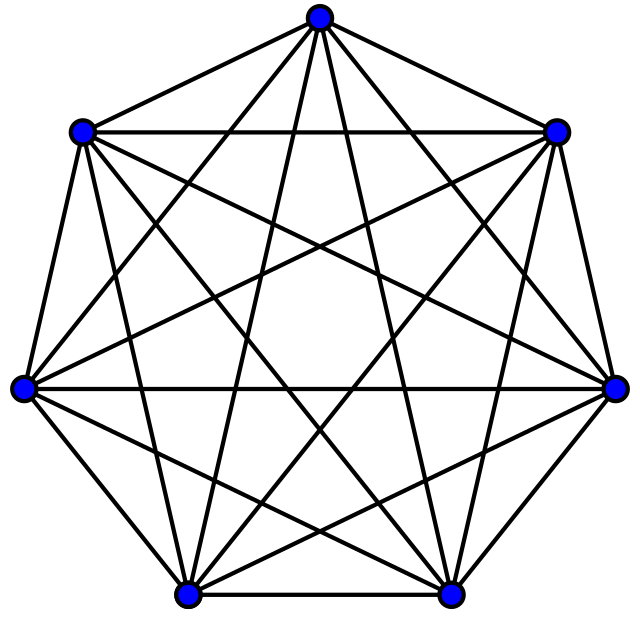
\includegraphics{complete-graph.png}
\caption{\emph{Image from Wikipedia}
A complete graph on 7 nodes has (7 * (7 -1))/2 = 21
edges}\end{figure}

We can find the number of edges a node's neighbors share by
examining the list of points that can be reached by two hops.
the node's neighbors will appear in this list once for each
edge they share with another neighbor. Therefore the number
of edges a node's neighbors share is the number of times it's
neighbors appear in the two hop list divided by two. Again
the division is necessary because both of an edge's end points
appear in the two hop list.
\begin{figure}[htbp]
\centering
\capstart

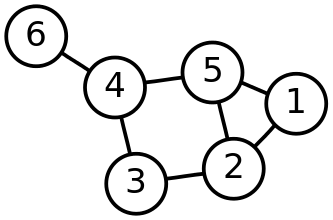
\includegraphics{open-graph.png}
\caption{\emph{Image from Wikipedia}}\end{figure}

In the above graph, 5's neighbors are 1, 2 and 4

3's two hop list is 2,5,1,3,5,3,5,6

1 and 2 each appear once so 5's neighbors share one edge
5's clustering coefficient is 1 / ((3 * (3-1))/2) = 1/3


\subsection{Writing the Algorithm}
\label{1-AdvancedNetwork/AdvancedNetwork:writing-the-algorithm}

\subsubsection{The Mapper}
\label{1-AdvancedNetwork/AdvancedNetwork:the-mapper}
First we will need to have a list of the friends and friends of
friends for every account. We can do this by sending each
account's list of friends to each of it's friends. We also
need to pass the account itself to the reducer so that it
will be able to build a list of it's friends. Here's the \code{code}

\begin{Verbatim}[commandchars=\\\{\},numbers=left,firstnumber=1,stepnumber=1]
\PYG{k}{def} \PYG{n+nf}{mapper}\PYG{p}{(}\PYG{n}{key}\PYG{p}{,} \PYG{n}{value}\PYG{p}{)}\PYG{p}{:}
  \PYG{n}{friends} \PYG{o}{=} \PYG{n}{value}\PYG{o}{.}\PYG{n}{split}\PYG{p}{(}\PYG{l+s}{'}\PYG{l+s}{,}\PYG{l+s}{'}\PYG{p}{)}
  \PYG{k}{for} \PYG{n}{friend} \PYG{o+ow}{in} \PYG{n}{friends}\PYG{p}{:}
    \PYG{n}{Wmr}\PYG{o}{.}\PYG{n}{emit}\PYG{p}{(}\PYG{n}{friend}\PYG{p}{,} \PYG{p}{(}\PYG{n}{key}\PYG{p}{,} \PYG{n}{value}\PYG{p}{)}\PYG{p}{)}
\end{Verbatim}

But what do we use as input? We already created friend
lists for each account in the last chapter. We could use this as
input for our clustering coefficient job. However this will
cause a few problems because WMR crashes when the values
the mappers emit are too large and some accounts have thousands of friends.
It's also not a good idea to have a single mapper
emitting a thousand values. We can get around these
limitations by breaking the friend lists into chunks before
we run the clustering coefficient job.

Our new friend list job uses the same \code{mapper}
as the one in the
last chapter, but a modified \code{reducer} that outputs 50 friends
at a time.

\begin{Verbatim}[commandchars=\\\{\},numbers=left,firstnumber=1,stepnumber=1]
\PYG{k}{def} \PYG{n+nf}{reducer}\PYG{p}{(}\PYG{n}{key}\PYG{p}{,} \PYG{n}{values}\PYG{p}{)}\PYG{p}{:}
  \PYG{n}{neighbors} \PYG{o}{=} \PYG{n+nb}{set}\PYG{p}{(}\PYG{p}{)}
  \PYG{k}{for} \PYG{n}{value} \PYG{o+ow}{in} \PYG{n}{values}\PYG{p}{:}
    \PYG{k}{if} \PYG{n+nb}{len}\PYG{p}{(}\PYG{n}{neighbors}\PYG{p}{)} \PYG{o}{\PYGZgt{}} \PYG{l+m+mi}{50}\PYG{p}{:}
      \PYG{n}{Wmr}\PYG{o}{.}\PYG{n}{emit}\PYG{p}{(}\PYG{n}{key}\PYG{p}{,} \PYG{l+s}{'}\PYG{l+s}{,}\PYG{l+s}{'}\PYG{o}{.}\PYG{n}{join}\PYG{p}{(}\PYG{n}{neighbors}\PYG{p}{)}\PYG{p}{)}
      \PYG{n}{neighbors} \PYG{o}{=} \PYG{n+nb}{set}\PYG{p}{(}\PYG{p}{)}
    \PYG{n}{neighbors}\PYG{o}{.}\PYG{n}{add}\PYG{p}{(}\PYG{n}{value}\PYG{p}{)}
  \PYG{k}{if} \PYG{n+nb}{len}\PYG{p}{(}\PYG{n}{neighbors}\PYG{p}{)} \PYG{o}{\PYGZgt{}} \PYG{l+m+mi}{0}\PYG{p}{:}
    \PYG{n}{Wmr}\PYG{o}{.}\PYG{n}{emit}\PYG{p}{(}\PYG{n}{key}\PYG{p}{,} \PYG{l+s}{'}\PYG{l+s}{,}\PYG{l+s}{'}\PYG{o}{.}\PYG{n}{join}\PYG{p}{(}\PYG{n}{neighbors}\PYG{p}{)}\PYG{p}{)}
\end{Verbatim}


\subsubsection{The Reducer}
\label{1-AdvancedNetwork/AdvancedNetwork:the-reducer}
Our \code{reducer} takes the lists of friends of friends and makes a
collection of it's one and two hop neighbors. We use a set for
the collection of one hop neighbors because we will receive
the same friend multiple times if it has a large friend list.

We will use a dict to store the number of times a node appears
in the two hop collection because it saves us a bit of memory
and allows us to avoid counting instances of an element in
a list which would be expensive.

\begin{Verbatim}[commandchars=\\\{\},numbers=left,firstnumber=1,stepnumber=1]
\PYG{k}{def} \PYG{n+nf}{reducer}\PYG{p}{(}\PYG{n}{key}\PYG{p}{,} \PYG{n}{values}\PYG{p}{)}\PYG{p}{:}
  \PYG{n}{oneHops} \PYG{o}{=} \PYG{n+nb}{set}\PYG{p}{(}\PYG{p}{)}             \PYG{c}{\PYGZsh{}friends}
  \PYG{n}{twoHops} \PYG{o}{=} \PYG{p}{\PYGZob{}}\PYG{p}{\PYGZcb{}}                \PYG{c}{\PYGZsh{}friends of friends}
  \PYG{k}{for} \PYG{n}{value} \PYG{o+ow}{in} \PYG{n}{values}\PYG{p}{:}
    \PYG{n}{node}\PYG{p}{,} \PYG{n}{hops} \PYG{o}{=} \PYG{n+nb}{eval}\PYG{p}{(}\PYG{n}{value}\PYG{p}{)}  \PYG{c}{\PYGZsh{}unpack the values}
    \PYG{n}{oneHops}\PYG{o}{.}\PYG{n}{add}\PYG{p}{(}\PYG{n}{node}\PYG{p}{)}         \PYG{c}{\PYGZsh{}reconstruct the friend list}
    \PYG{n}{hops} \PYG{o}{=} \PYG{n}{hops}\PYG{o}{.}\PYG{n}{split}\PYG{p}{(}\PYG{l+s}{'}\PYG{l+s}{,}\PYG{l+s}{'}\PYG{p}{)}
    \PYG{k}{for} \PYG{n}{hop} \PYG{o+ow}{in} \PYG{n}{hops}\PYG{p}{:}          \PYG{c}{\PYGZsh{}build the two hop dict}
      \PYG{k}{if} \PYG{n}{hop} \PYG{o+ow}{in} \PYG{n}{twoHops}\PYG{p}{:}
        \PYG{n}{twoHops}\PYG{p}{[}\PYG{n}{hop}\PYG{p}{]} \PYG{o}{+}\PYG{o}{=} \PYG{l+m+mi}{1}
      \PYG{k}{else}\PYG{p}{:}
        \PYG{n}{twoHops}\PYG{p}{[}\PYG{n}{hop}\PYG{p}{]} \PYG{o}{=} \PYG{l+m+mi}{1}
  \PYG{n}{n} \PYG{o}{=} \PYG{n+nb}{len}\PYG{p}{(}\PYG{n}{oneHops}\PYG{p}{)}
  \PYG{k}{if} \PYG{n}{n} \PYG{o}{\PYGZlt{}} \PYG{l+m+mi}{2}\PYG{p}{:}                   \PYG{c}{\PYGZsh{}if a point has less than 2}
    \PYG{n}{Wmr}\PYG{o}{.}\PYG{n}{emit}\PYG{p}{(}\PYG{n}{key}\PYG{p}{,} \PYG{l+m+mi}{0}\PYG{p}{)}          \PYG{c}{\PYGZsh{}neighbors it's cc is 0}
  \PYG{k}{else}\PYG{p}{:}
    \PYG{n}{total} \PYG{o}{=} \PYG{l+m+mf}{0.0}
    \PYG{k}{for} \PYG{n}{hop} \PYG{o+ow}{in} \PYG{n}{oneHops}\PYG{p}{:}
      \PYG{k}{if} \PYG{n}{hop} \PYG{o+ow}{in} \PYG{n}{twoHops}\PYG{p}{:}
        \PYG{n}{total} \PYG{o}{+}\PYG{o}{=} \PYG{n}{twoHops}\PYG{p}{[}\PYG{n}{hop}\PYG{p}{]}
    \PYG{n}{cc} \PYG{o}{=} \PYG{n}{total} \PYG{o}{/} \PYG{p}{(}\PYG{n}{n} \PYG{o}{*} \PYG{p}{(}\PYG{n}{n}\PYG{o}{-}\PYG{l+m+mi}{1}\PYG{p}{)}\PYG{p}{)}  \PYG{c}{\PYGZsh{}calculate the cc}
    \PYG{n}{Wmr}\PYG{o}{.}\PYG{n}{emit}\PYG{p}{(}\PYG{n}{key}\PYG{p}{,} \PYG{n}{cc}\PYG{p}{)}
\end{Verbatim}


\subsection{Challenge exercises for you to try}
\label{1-AdvancedNetwork/AdvancedNetwork:challenge-exercises-for-you-to-try}\begin{enumerate}
\item {} 
Calculate the average value of the clustering coefficient.

\end{enumerate}
\begin{quote}

Can you reuse the code from the last exercise?
\end{quote}
\begin{enumerate}
\setcounter{enumi}{1}
\item {} 
Develop a chain of jobs to count the number of triangles

\end{enumerate}
\begin{quote}

in the network. (Hint: pick a point to be the tip of
the triangle)
\end{quote}
\begin{enumerate}
\setcounter{enumi}{2}
\item {} 
Using code from the previous challenge, come up with

\end{enumerate}
\begin{quote}

another way of calculating the clustering coefficient.
You can test your algorithm by comparing the average
with the average you calculated in the first challenge.
\end{quote}



\renewcommand{\indexname}{Index}
\printindex
\end{document}
